\documentclass[a4paper][11pt][titlepage]{article}

\usepackage{color}
\usepackage[dvipdfm]{graphicx}
\usepackage{identfirst}


\begin{document}
\begin{titilepage}

\begin{figure}[t]  
  
\includegraphics{Imperial-College-logo.png}
\end{figure}

\title{What are the roles of CRISPR and Anti-CRISPR system in the dynamic of bacteria and bacteriophage in the infant gut?}
\author{Jiqiu Wu\\j.wu18@imperial.ac.uk}
\date{Dec 2018}

\begin{center}
Supervisor: Tim G. Barraclough t.barraclough@imperial.ac.uk Imperial College London\\ Stineke Van Houte c.van-houte@exeter.ac.uk The University of Exeter\\Edze Westra e.r.westra@exeter.ac.uk The University of Exeter\\
\end{center}
\end{titilepage}


			

			
			
}
}
			
\end{titlepage}

  
  \begin{abstract}
    
  
  Gut microbiota, composed by bacteria, fungi and viruses, play an essential role 
  in the health of human and animals. Gut microbiota in infant can take effort to 
  the gut development in adult. There is a dynamic process between bacteria and 
  bacteriophages in early life, however, the interaction between the two important 
  composition is unclear. In this project, we will use computational methods to study 
  if CRISPR and Anti-CRISPR take part in the process and what the role it takes based 
  on data from public database. 

  Keywords: Infant gut microbiota CRISPR Anti-CRISPR
  \end{abstract}
  
  \section{Introduction}
   The mammalian microbiome consists of bacteria, archaea, fungi and viruses.\cite{Lynch2016}
    They have a profound influence on human physiology, nutrition and disease.\cite{Qin2010}
    They form a bioreactor and produce bioactive compounds. 
   These compounds signal to distant organs including brain, liver, heart,
   lung and so forth.\cite{Schroeder2016} In heart, gut micro-derived metabolites are recognized 
   as contributors to atherogenesis.\cite{wang2011gut}  Microbiomes play a role in neurodevelopmental 
   and mood disorders.\cite{de2014food} Differences in species richness and their diversity between 
   autism spectrum disorder (ASD) and controls have been reported.\cite{williams2012application} As one part of the 
   gut microbiome, the virome has a significant implication in health and disease.\cite{virgin2014virome} during
    inflammatory bowel diseases(IBD) the intestinal phage population is altered and 
    transitions from an ordered state to a stochastic dysbiosis in murine.\cite{duerkop2018murine}

    The microbiota of infants is a key factor for the development of the microbiome.\cite{stewart2018temporal}
    Epidemiological studies have shown that factors that alter bacterial communities in 
    infants during childhood increase the risk for several diseases.\cite{tamburini2016microbiome} Childhood overweight 
    is associated with the microbiota of early life in Denmark\cite{ajslev2011childhood} and Norway\cite{stanislawski2018gut}. Early gut
     microbiota was associated with infant growth rates.\cite{white2013novel} As for immune system, a diverse 
     early life intestinal microbiota can inhibit the pathways that lead to allergic 
     sensitization by multiple mechanisms.\cite{reynolds2017early} Besides, researches over the past few years 
     reveal that the gut microbiome plays a role in basic neurogenerative processes and 
     modulates many aspects of animal behavior in early life.\cite{sharon2016central}

     The ecology of the bacterial microbiome increases in richness and diversity towards 
     an adult-like composition.\cite{yatsunenko2012human} Soon after birth, the bacterial microbiome rapidly switches 
     from predominantly facultative anaerobic bacteria to a diverse community of anaerobes.\cite{koenig2011succession}
     During the first months of life, the early infant gut bacteriophage virome is composed of 
     a rich community of bacteriophages, the majority of which derive from the Caudovirales 
     order. Subsequently, the bacteriophages decrease in richness and shifts towards a 
     Microviridae-dominated community over the first 2 years of life. Thus, the infant virome 
     and bacterial microbiome evolves in a dynamic trajectory during the early years of life.\cite{lim2015early}

     As the Red Queen hypothesis proposes that organisms must continually evolve new 
     mechanisms of resistance to parasites to avoid extinction.\cite{liow2011red} Bacteria have evolved 
     a great of diverse strategies to defend themselves against phage, including 
     restriction–modification enzymes that inactivate target DNA by cleavage, toxin–antitoxin 
     modules that lead to phage abortive infection and CRISPR–Cas systems that target and 
     inactivate specific nucleic acid sequences by cleavage. In response, phages have evolved 
     various mechanisms to overcome these defenses, including expression of proteins that 
     modify restriction sites\cite{kruger1983bacteriophage} or degrade restriction– modification cofactors\cite{studier1976samase}, antitoxin 
     molecules that inhibit the activity of toxin‑antitoxin abortive infection systems\cite{otsuka2012dmd} and 
     proteins that directly bind to and inactivate CRISPR–Cas machinery\cite{pawluk2016naturally}.

     Thus, CRISPR-Cas and anti-CRISPR of the metagenomic and 16S rRNA sequences from eight 
     healthy infants (four twin pairs) between 0-2 years old \cite{lim2015early} will be studied. Computational 
     approaches will be used to detect CRISPR-Cas and anti-CRISPR sequences. What kind of 
     CRISPR-Cas and anti-CRISPR are contained and during the dynamic process of bacteria-
     bacteriophage, if the CRISPR and Anti-CRISPR systems change, if they play a role will 
     be answered. If the switch of lysogenic and lytic life style drives the dynamic process 
     will be studied. Besides, in terms of previous researches, there is no CRISPR system in 
     Bacteroidetes and no anti-CRISPR in Caudovirales62 which are dominant in gut, new insight 
     is wished. 

     Extrally, Maybe we can study the known interactions between anti-CRISPR proteins 
     and their binding site of CRISPR-Cas, and then predict the novel anti-CRISPR proteins 
     based on the numerous CRISPR-Cas data.\cite{alipanahi2015predicting}
  
  \section{Materials \& Methods}  
  Customized metagenomic and 16S rRNA sequences from eight healthy infants (four twin 
  pairs) between 0-2 years old\cite{lim2015early} can be downloaded. Some operations have been done 
  previous researchers. And the methods of virome sequencing processing, virome analysis 
  and 16S rRNA gene analysis have been described.32 And the Methods of CRISPR analysis including 
  indentification CRISPR spacers and indentification of phage contifs have been described.\cite{stern2012crispr} 
  As for Anti-CRISPR analysis, There are two strategies for detecting Anti-CRISPR. First, 
  using the Anti-CRISPR database 65 to query the metagenomic data using BLASTN with e-value 
  threshold of 1E-4. Second, using the aca gene sequences combined from all the previous 
  researches to query the metagenomic data using the same parameters. There are two principles\cite{stern2012crispr} 
  that can lead to the Python script for detection of the lysogenic phages. First, the lysogenic 
  phages should be combined with integrase and recombinase. Second, the lysogenic phages 
  should be integrated into bacteria with flanking sequences. And for the left phages, 
  we regard them as lytic phages.

	\begin{figure}[h]  
  \centering
			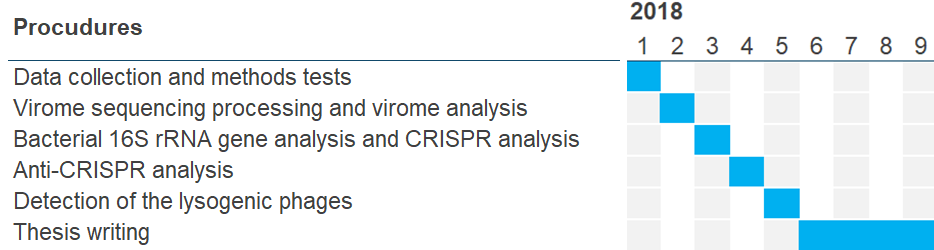
\includegraphics{gatt.png}
      \caption{Gantt Chart}
      \end{figure}
    
    
  


	
	
	
	\section{Budget}
	
	Probably, this project don't need budget.
    
    Supervisor Tim G. Barraclough, Stineke Van Houte and Edze Westra has seen and accepted 
    budget.
  
  \bibliographystyle{plain}
  \bibliography{proposal}
\end{document}
\grid